\section{Mockups}
	Mockups for the mobile and web application have been presented and discussed in the RASD. 

\section{UX Diagrams}
	In this section User eXperience diagrams are presented with the intent of defining UI's screens and their interactions.
	\\As stated in the RASD web and mobile application are almost identical and will be treated as a unique application from the UX point-of-view.

	\subsection{On-Board application}
		\begin{figure}[!ht]
		  \centering
		  \vspace{0.2cm}
		  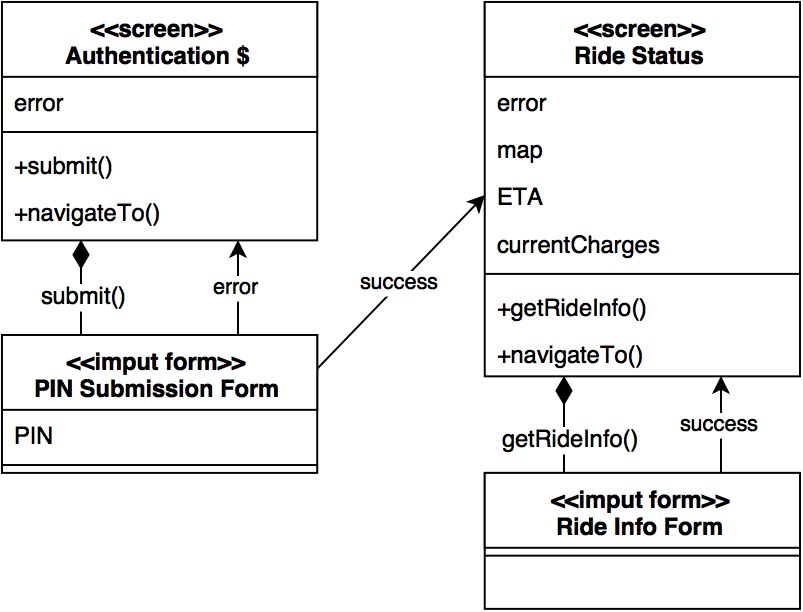
\includegraphics[width=0.4\textwidth]{/DD/OB_ux_schema}\\
		  \vspace{0.4cm}
		  \caption{UX scheme for the on-board application} 
		  \label{fig:OB_ux_scheme} 
		\end{figure}

		After authenticating using his Personal Identification Number, a screen is displayed to the user containing the ride-status informations (which are continuously refreshed through 'getRideInfo').


	\subsection{Mobile/Web application}
		\begin{figure}[!ht]
		  \centering
		  \vspace{0.2cm}
		  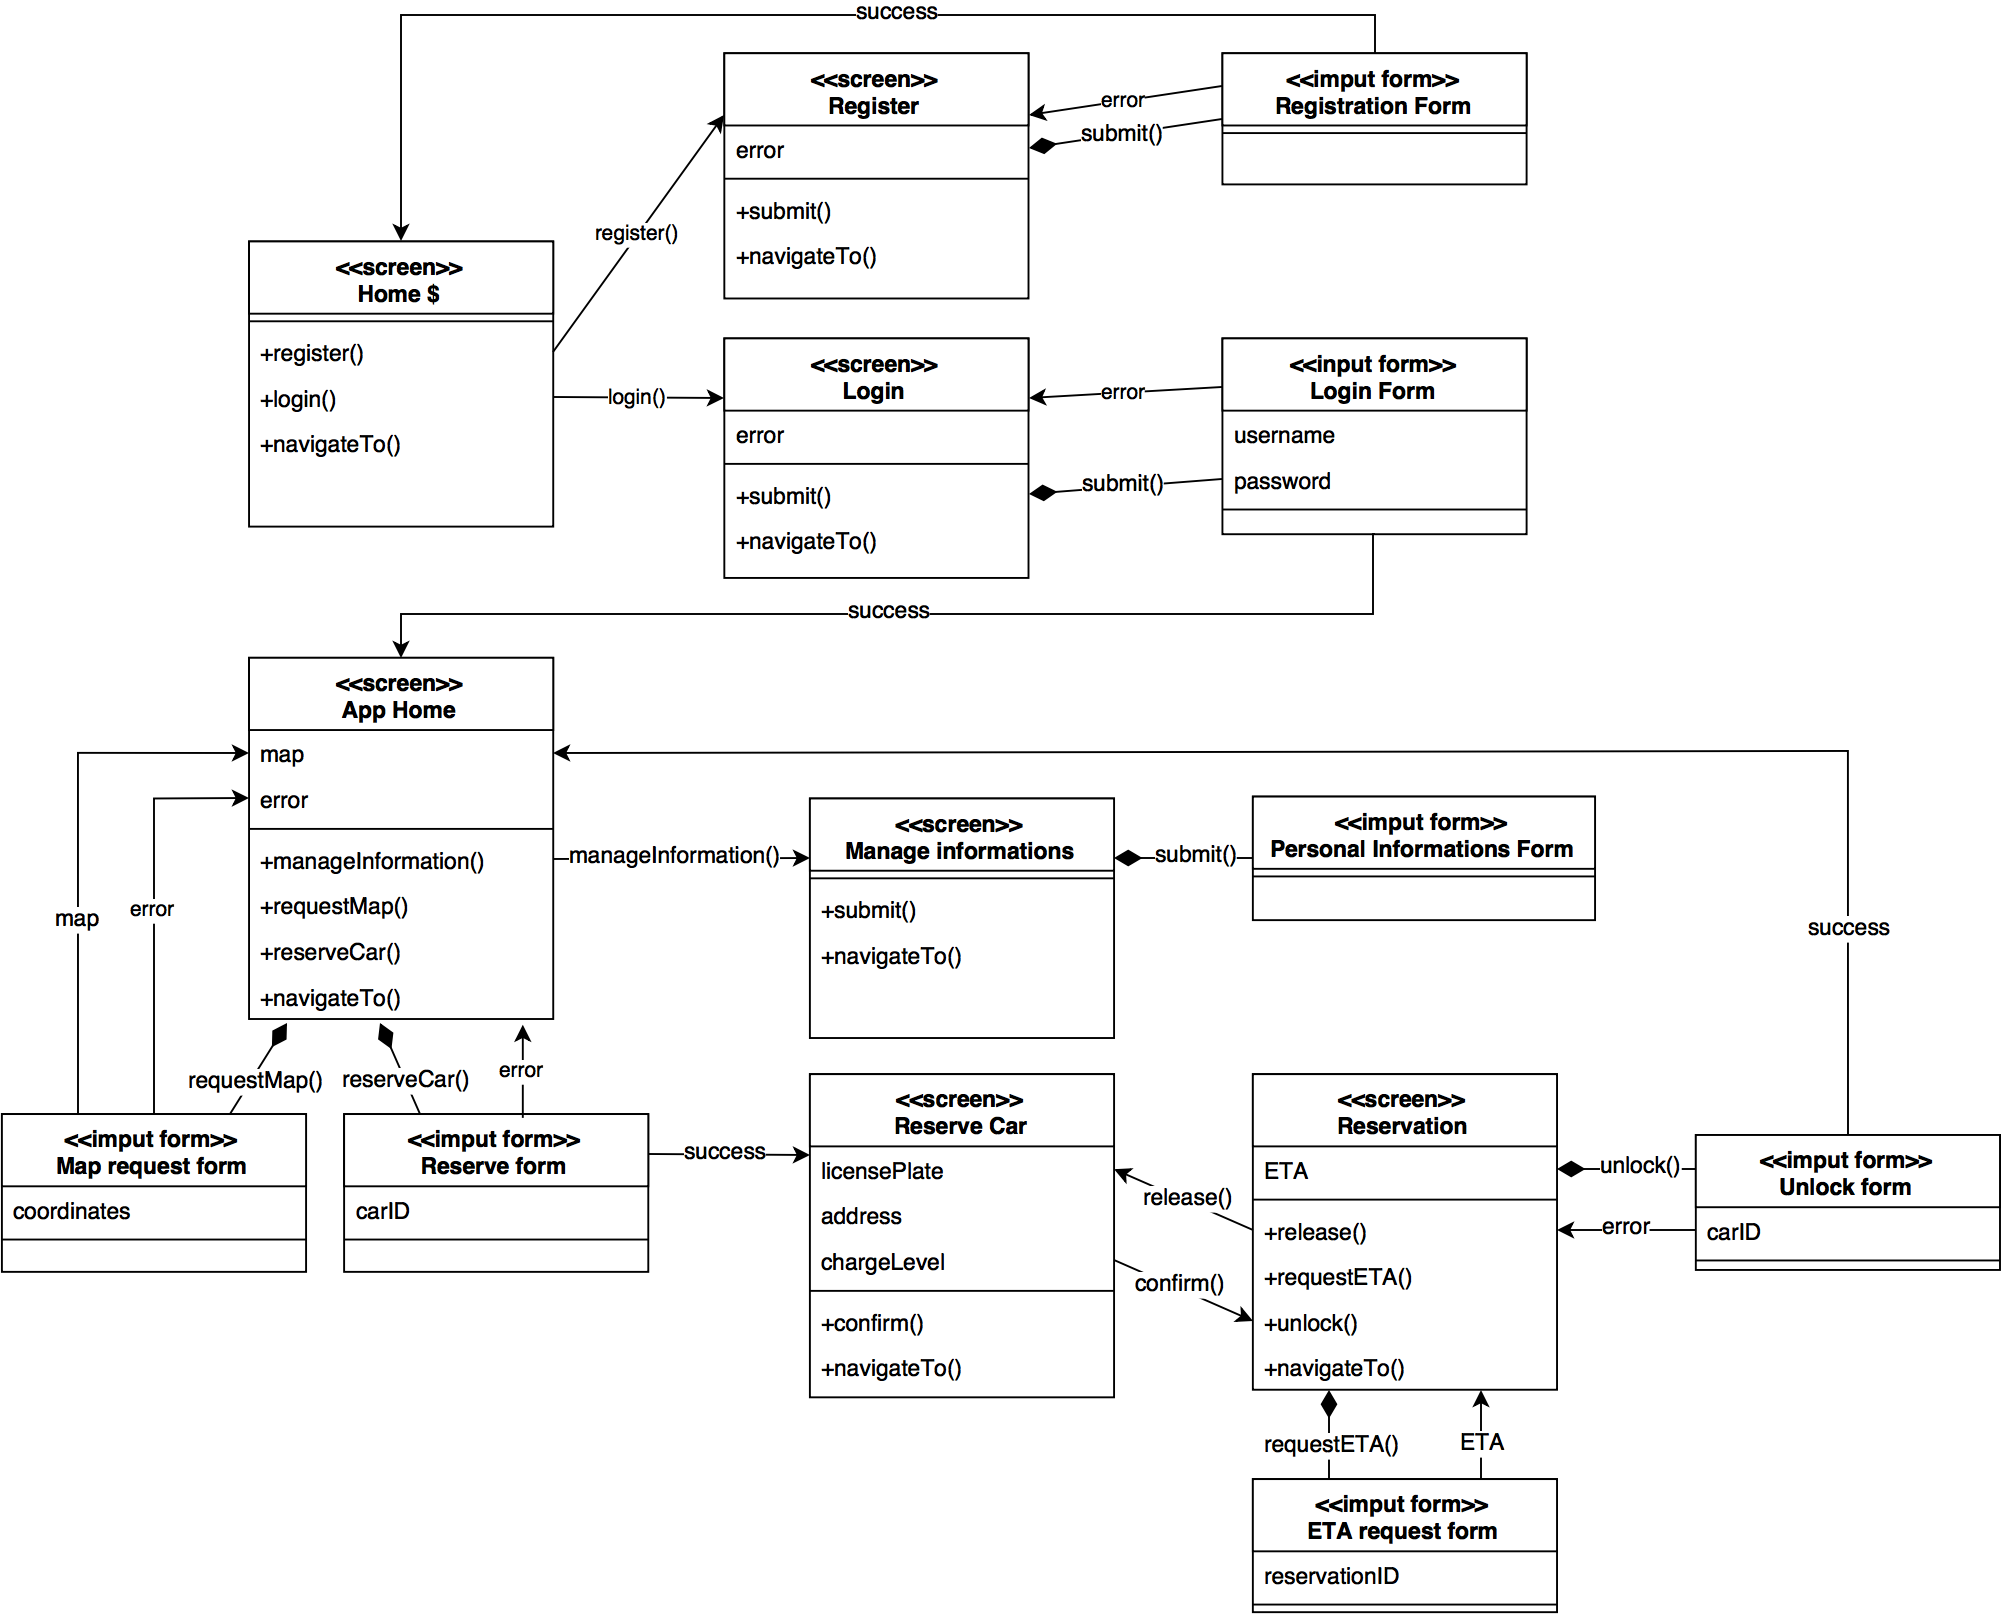
\includegraphics[width=1.0\textwidth]{/DD/ux_schema}\\
		  \vspace{0.4cm}
		  \caption{UX scheme for the mobile and web applications} 
		  \label{fig:ux_scheme} 
		\end{figure}

		After the registration/login the app home page is presented: this screen comprehend a map where all the available cars, safe area and charging stations (which are contained in the 'map' object and continuously refreshed through 'requestMap') are displayed. The user can either navigate to the 'Manage Informations' screen (where he can consult and edit his personal informations) or reserve a car after selecting it on the map. The car is tagged as 'RESERVED' after the user's confirmation and then a 'Reservation' screen is displayed: a timer shows up and the user can Release the reservation or proceed with the Unlock.
		\\When the ride ends the payment is automatically authorized and processed without any user action.
